\documentclass[draftcls,onecolumn]{IEEEtran}
%%%%%%%%%%%%%%%%%%%%%%%%%%%%%%%%%%%%%%%%%%%%%%%%%%%%%%%%%%%%%%%%%%%%%%%%%%%%%%%%
%                                                                              %
%                                   PREAMBLE                                   %
%                                                                              %
%%%%%%%%%%%%%%%%%%%%%%%%%%%%%%%%%%%%%%%%%%%%%%%%%%%%%%%%%%%%%%%%%%%%%%%%%%%%%%%%
%% INCLUDING THE PREAMBLE
%%%%%%%%%%%%%%%%%%%%%%%%%%%%%%%%%%%%%%%%%%%%%%%%%%%%%%%%%%%%%%%%%%%%%%%%%%%
%                                                                         %
%                                 PREAMBLE                                %
%                                                                         %
%%%%%%%%%%%%%%%%%%%%%%%%%%%%%%%%%%%%%%%%%%%%%%%%%%%%%%%%%%%%%%%%%%%%%%%%%%%

%% PACKAGES
\usepackage[]{lineno}
%\linenumbers
\usepackage[usenames,dvipsnames]{xcolor}
\usepackage{microtype}
\usepackage[obeyDraft]{todonotes}
\usepackage{fancyvrb}
\VerbatimFootnotes
\usepackage{algorithmic}

%% GRAPHICS RELATED
\usepackage{graphicx}
\usepackage[outdir=./tmp/]{epstopdf}
\graphicspath{{../images/}{./}{./tmp/}}
\DeclareGraphicsExtensions{.eps, .pdf, .jpeg, .png,}

%% CPATION SETUP
\usepackage{float}
\usepackage{caption}
\usepackage{subcaption}
\captionsetup{belowskip=12pt,aboveskip=4pt}


%% BIBLIOGRAPHY
\bibliographystyle{ieeetr}

%% UNITS
\usepackage{siunitx}

%% EQUATIONS
\usepackage{amsmath}
%\numberwithin{equation}{section}

%% HYPERLINKS
\usepackage[debug]{hyperref}

%%%%%%%%%%%%%%%%%%%%%%%%%%%%%%%%%%%%%%%%%%%%%%%%%%%%%%%%%%%%%%%%%%%%%%%%%%%
%                                                                         %
%                             Listing Setup                               %
%                                                                         %
%%%%%%%%%%%%%%%%%%%%%%%%%%%%%%%%%%%%%%%%%%%%%%%%%%%%%%%%%%%%%%%%%%%%%%%%%%%
\usepackage{listings}
\lstset{ %
    language=C++,
    basicstyle=\footnotesize\ttfamily,
    numbers=left,
    numberstyle=\tiny\color{gray},
    stepnumber=2,
    numbersep=5pt,
    backgroundcolor=\color{white},
    showspaces=false,
    showstringspaces=false,
    showtabs=false,
    frame=single,
    rulecolor=\color{black},
    tabsize=2,
    breaklines=true,
    breakatwhitespace=false,
    title=\lstname,
    keywordstyle=\color{blue},
    commentstyle=\color{OliveGreen},
    stringstyle=\color{orange}
}
\DeclareCaptionFont{white}{\color{white}}
\DeclareCaptionFormat{listing}{\colorbox[cmyk]{0.43, 0.35, 0.35, 0.01}{\parbox{\dimexpr\textwidth-2\fboxsep\relax}{#1#2#3}}}
\captionsetup[lstlisting]{format=listing,labelfont=white,textfont=white,singlelinecheck=false,margin=0pt,font={bf,footnotesize}}
%\lstnewenvironment{code}[1][]%
%{ \noindent\minipage{\linewidth}
%	\lstset{#1}
%}
%{\endminipage}
%% USER COMMANDS
\usepackage{isotope}
\newcommand{\iso}{\isotope}
\newcommand{\figurewidth}{\textwidth}
\newcommand{\micron}{$\mu$m}


\usepackage{standalone}
\graphicspath{{./images/}{./}}
\DeclareGraphicsExtensions{.pdf, .jpeg, .png, .jpg}
% TO COMPILE: lmake
%%%%%%%%%%%%%%%%%%%%%%%%%%%%%%%%%%%%%%%%%%%%%%%%%%%%%%%%%%%%%%%%%%%%%%%%%%%%%%%%
%                                                                              %
%                               START OF DOCUMENT                              %
%                                                                              %
%%%%%%%%%%%%%%%%%%%%%%%%%%%%%%%%%%%%%%%%%%%%%%%%%%%%%%%%%%%%%%%%%%%%%%%%%%%%%%%%
\begin{document}

% Cover Page
\title{Moderation of Neutron Sources with HDPE}
\author{Matthew J. Urffer}

\maketitle
\begin{abstract}
The moderation of neutrons by high density polyethylene (HDPE) is invistigated as a function of source energy and thickness of HDPE.
MCNP was used to simulate the neutronics for a point neturon source, as well as a \isotope[252]{Cf} source for thickness ranging from 0.5 cm to 32 cm (\~ 1 foot).
A series of curves were constructed in order to present this data.
\end{abstract}

\IEEEpeerreviewmaketitle

% To Do List
\listoftodos
\pagebreak
% Tables of Contents, Figures, Tables
\tableofcontents
\pagebreak
\listoffigures
\pagebreak
\listoftables
\pagebreak
\lstlistoflistings

\section{Introduction}
Understanding the moderation of neutrons is essential in neutron detectors designs.
Many of the neutron detection reactions have a much larger (by orders of magnitudes) probability of occurance if the neutrons are thermal.
Thus, great effort is taken to moderate the neutron spectra in order to increase the probability of a desired reaction to occur.
High density polyethelene (HDPE) is a well known neutron moderator with a denisty ranging from $0.93 g/cm^3$ to $0.97 g/cm^3$.
Polyethelene,$\left (C_2 H_4\right )_n H_2$, has four hydrogen atoms per repeating unit making it an ideal neutron moderator because each neutron can lose almost all of it's energy upon an elastic collision with a hydrogen atom given that the hydrogen atom and neutron have similar masses.
HDPE is also stable at room temperature, non-toxic, and has enough strucutral integrity that one can build with it.

This work will focus on the moderation of two types of neutron sources; a mono energic point source of various energies and a \iso[252]{Cf} source.
For both sources the thickness of HDPE encasing the source is varied, and the fraction of thermal neutrons is calcualted.


This paper is organzied into the following sections.  The Methods section will outline the geometry used for the MCNP simulation, as well as an indepth explanation of how the fraction of thermal neutrons was calculated.  The Results section will outline the pertiant results, with the Conclusions section summerizing the work.

%%% Methods Section
\section{Methods}

In the case of the mono energic point source the source is directly surrounded by HDPE, as shown in Figure ~\ref{fig:PointSrcGeo}. 
The \iso[252]{Cf} source is not presented as a bare point source.
Rather, the source is modeled as as a point \iso[252]{Cf} source sournded by 0.5 cm of lead. The lead sphere is then encased in HDPE as shown in Figure ~\ref{fig:Cf252SrcGeo}.
In both source configurations the source is taken to be isotropic. 
For the point source was modeled for neutron energies of 1 eV, 1 keV, and 1 MeV.
The \iso[252]{Cf} source was modeled using the spontanous fission spectra built into MCNPX.
\begin{figure}
  \centering
  \begin{subfigure}[b]{0.45\textwidth}
    \centering
    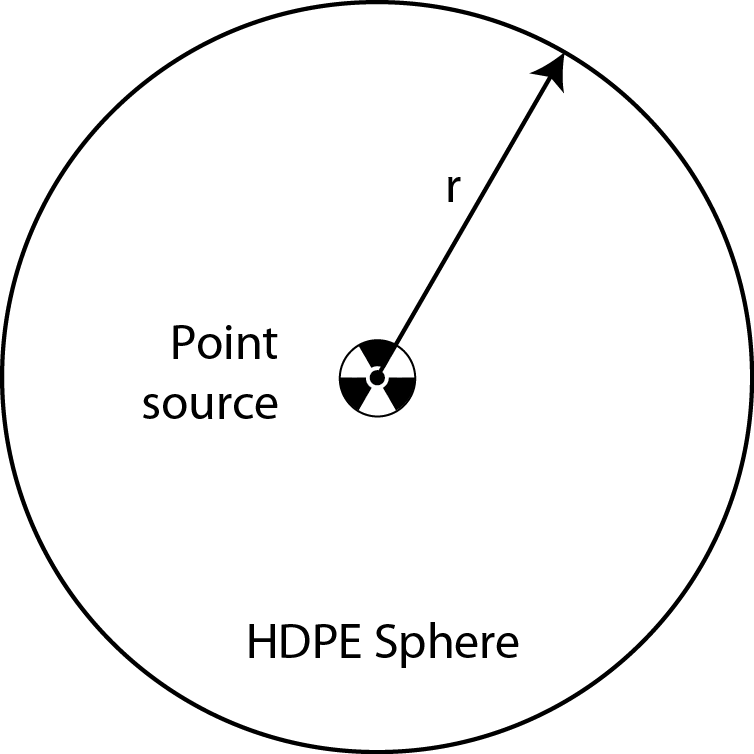
\includegraphics[width=\textwidth]{HDPEModeration_PointSrcGeo}
    \caption{Geometry of mono energetic point source}
    \label{fig:Cf252SrcGeo}
  \end{subfigure}%
  ~
  \begin{subfigure}[b]{0.45\textwidth}
    \centering
    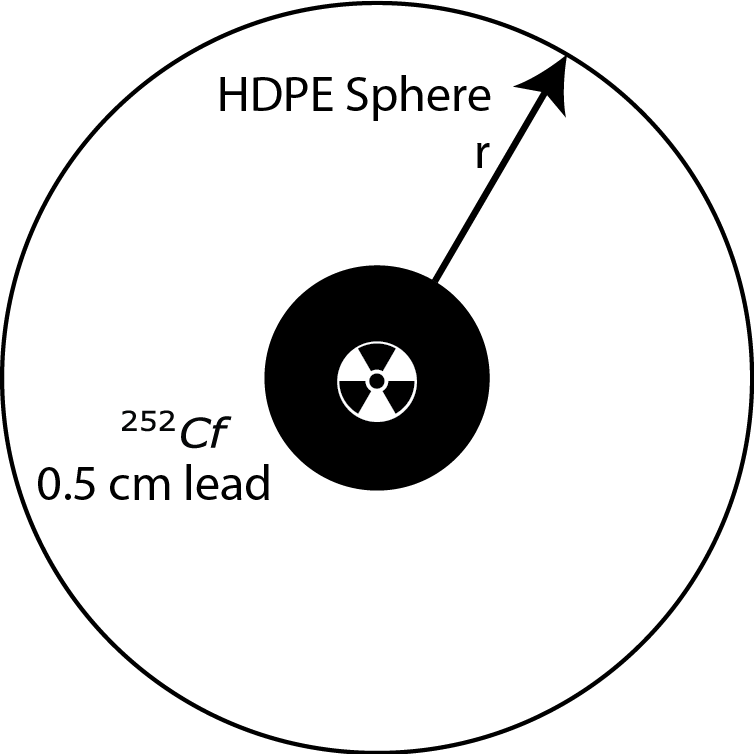
\includegraphics[width=\textwidth]{HDPEModeration_Cf252SrcGeo}
    \caption{Geometry of \isotope[252]{Cf} source}
    \label{fig:Cf252SrcGeo}
  \end{subfigure}
  \caption{Simulated Geometry}
\end{figure}

The thermal fraction is defined in \eqref{eqn:ThermalFraction} and was calculated by bining into two energy bins seperated by $5\times10^{-7}\text{MeV}$ (0.5 eV), normalizing by the total flux.
The thermal energy of 0.5 eV was chosen because this is the close to the cadmium cutoff.
\begin{align}
    \label{eqn:ThermalFraction}
    \eta = \frac{\int_0 ^{E_\text{termal}} \phi(E)dE}{\int_0^\infty \phi(E)dE}
\end{align}

\subsection{Simulation}
The neutronic simulations were completed in MCNPX. 
A generic MCNPX input deck was written for the point source (Listing ~\ref{lst:PointSrcScript}) and for the \iso[252]{Cf} source (Listing ~\ref{lst:Cf252SrcScript}).
A BASH script was then written in order to run multiple jobs, using \verb+sed+ to preform in place edits of the files.
For the point source this invovled itterating through a list of energies and then a list of distances.
The \iso[252]{Cf} source only involved itterating through a list of distances.
These scripts are shown in Listing ~\ref{lst:PointSrcRUNDATA} and Listing ~\ref{lst:Cf252SrcRUNDATA}.


%%% Results Section
\section{Results}
\label{sec:Results}
\begin{figure}[!ht]
	\centering
	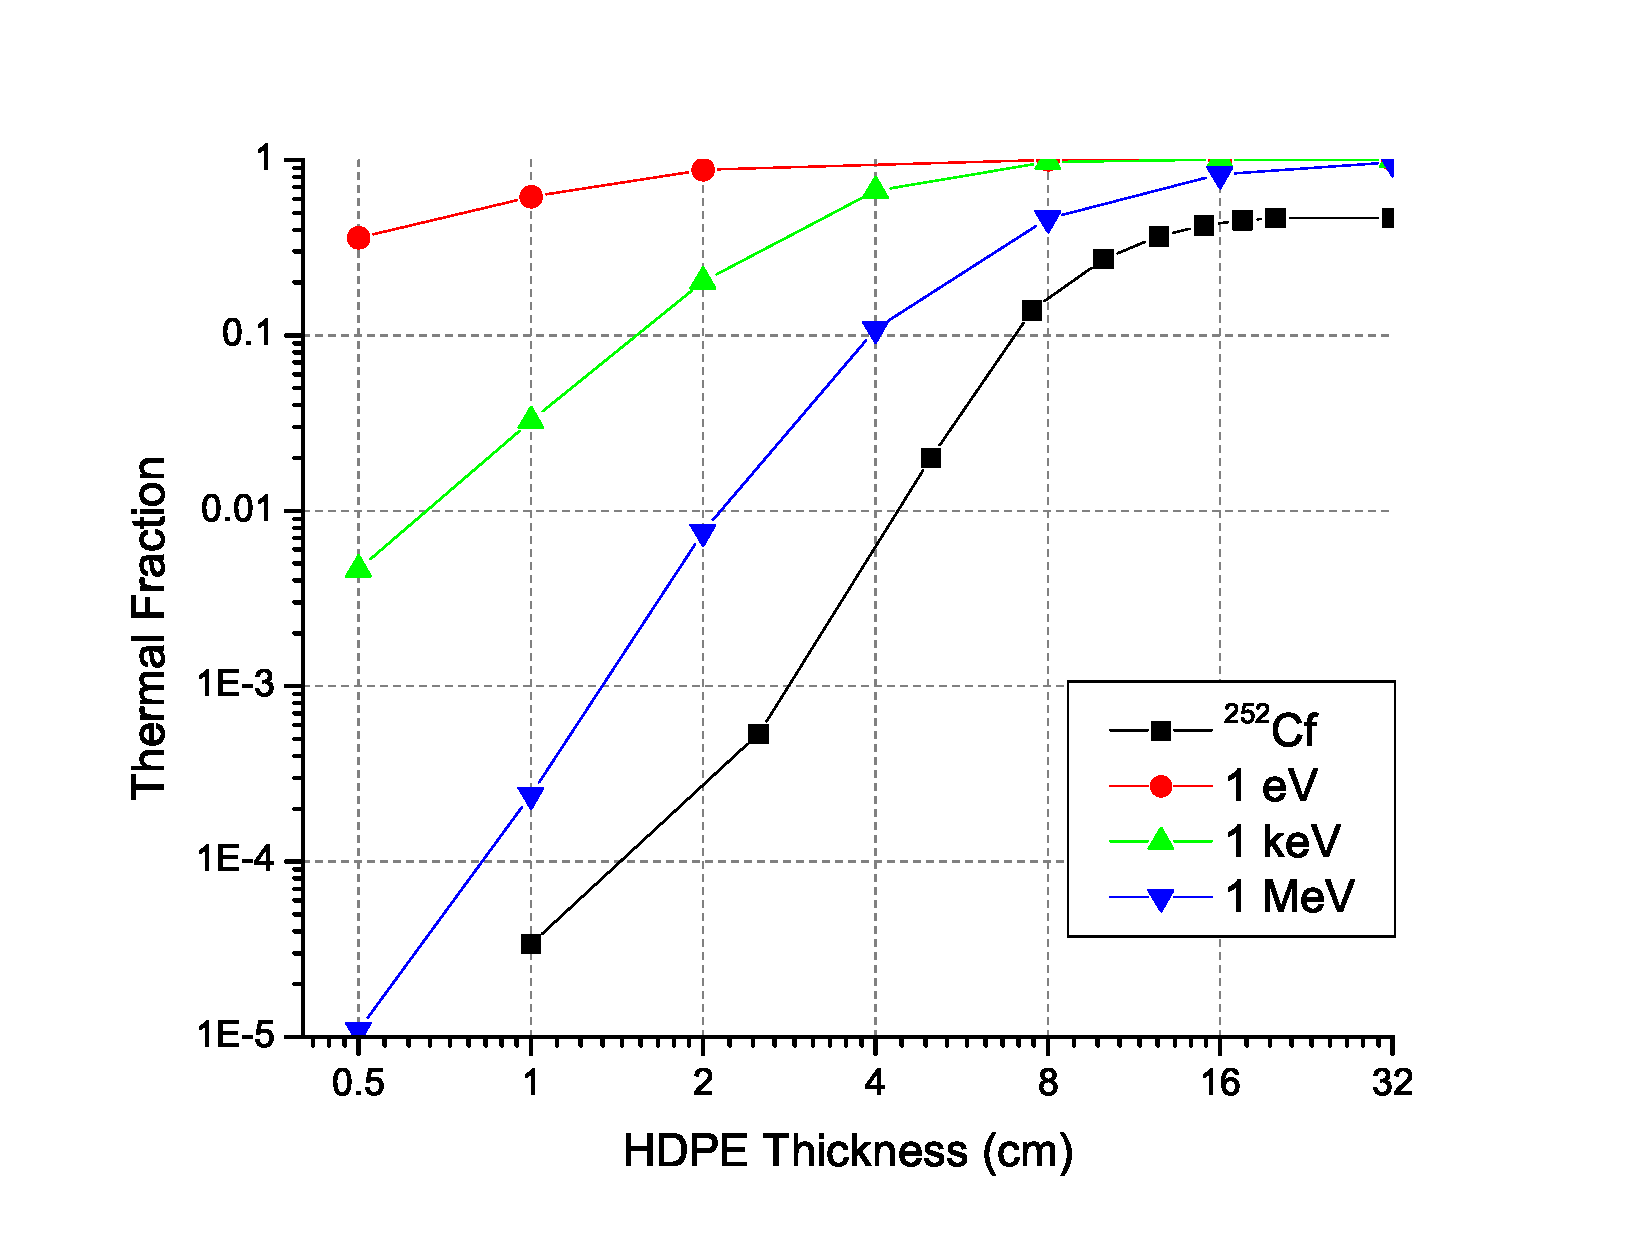
\includegraphics[width=\textwidth]{HDPEModThermalFraction}
	  \caption{Thermal Neutron Fraction}
	  \label{fig:ThermalNeutronFraction}
\end{figure}
The MCNPX results were post processed in order to compute the fraction of neutrons that are thermal according to \eqref{eqn:ThermalFraction}.
The results are displayed in  Figure ~\ref{fig:ThermalNeutronFraction}.
For low energies (below \SI{1}{\kilo\electronvolt}) the fraction of thermalization does not depend highly on the moderator thickness as the most of the neutrons are moderated within a few collisions in the materials.
For the 1 MeV neutrons about 10 \% of the neutrons thermalized in 4 cm, approaching an asymptote around 16 cm (though about 50\% are thermailzed after 8 cm).
The \iso[252]{Cf} source (because of MeV range tail) does not become thermalized as quickly.
Rather, it takes about 8 cm of HDPE in order to thermalize the spectra to 10\%. 
At around 16 cm the \iso[252]{Cf} spectra reaches it's asymptote of around 50\% thermalize.


% Bibliography
\bibliography{./Zotero}

\appendix
%%%%%%%%%%%%%%%%%%%%%%%%%%%%%%%%%%%%%%%%%%%%%%%%%%%%%%%%%%%%%%%%%%%%%%%%%%%%%%%%%
%                                                                              %
%                                   PREAMBLE                                   %
%                                                                              %
%%%%%%%%%%%%%%%%%%%%%%%%%%%%%%%%%%%%%%%%%%%%%%%%%%%%%%%%%%%%%%%%%%%%%%%%%%%%%%%%
% TO COMPILE: pdflatex
\documentclass[draftcls,onecolumn]{IEEEtran}
\usepackage{listings,graphicx,amsmath}
\usepackage{microtype,todonotes}
\usepackage{isotope}

%% BIBLIOGRAPHY
\bibliographystyle{ieeetr}

%% GRAPHICS RELATED
\usepackage{graphicx}
\usepackage{listings,amsmath}
\graphicspath{{./images/}{./}}
\DeclareGraphicsExtensions{.pdf, .jpeg, .png, .jpg}

%% CAPTION SETUP
\usepackage{float}
\usepackage{caption}
\usepackage{subcaption}
\captionsetup{belowskip=12pt,aboveskip=4pt}

% *** CITATION PACKAGES ***
\usepackage{cite}

% *** SPECIALIZED LIST PACKAGES ***
\usepackage{algpseudocode}
\usepackage{algorithm}
\algnewcommand{\algorithmicgoto}{\textbf{go to}}%
\algnewcommand{\Goto}[1]{\algorithmicgoto~\ref{#1}}

\usepackage{hyperref}

% *** ALIGNMENT PACKAGES ***
\usepackage{array}
\usepackage{pgfplotstable}
%%%%%%%%%%%%%%%%%%%%%%%%%%%%%%%%%%%%%%%%%%%%%%%%%%%%%%%%%%%%%%%%%%%%%%%%%%%%%%%%
%                                                                              %
%                               START OF DOCUMENT                              %
%                                                                              %
%%%%%%%%%%%%%%%%%%%%%%%%%%%%%%%%%%%%%%%%%%%%%%%%%%%%%%%%%%%%%%%%%%%%%%%%%%%%%%%%

\begin{document}

% paper title
\title{Moderation of HDPE source}

% author names and affiliations
%\author{\IEEEauthorblockN{Matthew J. Urffer}
%matthew.urffer@gmail
%}

\maketitle


\IEEEpeerreviewmaketitle

% Sections (Other Documents)
\section{Introduction}
A 2.4 MeV D-D neutron source of $1.2\times 10^{12}$ n/s or a 14.1 MeV D-T neutron source of $3.5\times10^{14}$ n/s is desired to be moderated to thermal energies with a thermal flux on the order of $10^{7} n/cm^2s$.
Thermal energies were defined to be energies below $1\times10^{-7}$ MeV or 100 meV.
A brief literature review suggest that a large amount of moderator is needed  in order to decrease the ratio of the fast neutron flux to thermal flux (RFNT) as shown in the reproduced published results (Figure ~\ref{fig:Fig2Paper}).
It should be noted that the fraction of thermal neutrons is not the same as the RFNT, but demonstrates that the amount of moderator needed is on the order of 50-100 cm.
\begin{figure}
	\centering
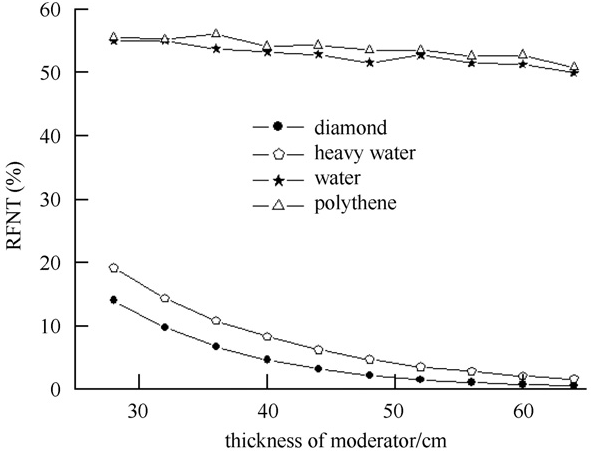
\includegraphics[width=0.5\textwidth]{DTModeratorFig2}
\caption{Fraction of Spectra Thermalized}
\label{fig:Fig2Paper}
\end{figure}

\section{Methods}
\subsection{Geometry and MCNP Simulation}
The geometry was modeled as a point source of the energies of the D-D reaction (2.4 MeV) and of the D-T reaction (14.1 MeV).
The source was then surrounded by a sphere of HDPE, with the detector being another sphere concentric with the HDPE moderator (encompassing 4$\pi$ steradians).
The neutronics was calculated with MCNP. Two tallies were employed:
\begin{itemize}
    \item Current tally (F1) over the source to ensure correct energy distribution.
    \item Current tally (F1) over the edge of the HDPE to calculate moderation.
    \item Flux tally (F2) over detector boundary to calculate the moderated flux.
\end{itemize}
The tally normalization was left as the MCNP results; i.e. no normalization on the F1 tally, and normalized by the surface area for the F2 surface flux tallies.
This allowed for the easy verification of the source distribution (a spike of 1.0 at the source energy), and for the amount of neutrons absorbed in the moderator to be easily calculated \footnote{MCNP reports on a per source particle basis, leaving it up to the user to correct for the source strength.}.

The fraction of  thermal neutrons is calculated as follows:
\begin{equation}
\eta = \frac{\int_{0}^{1\times10^{-7} MeV} \phi(E)dE}{\int_0^{\infty}\phi(E)dE}
\end{equation}
The validity of this calculation was checked by computing the fraction of thermal neutrons for neutron energies from the \isotope[252]{Cf} spontaneous fission spectra - \isotope[252]{Cf} spontaneous fission spectra has the most probable energy of 0.7 MeV with the average of 2.1 MeV.
As shown in Figure ~\ref{fig:FractionThermalized} for low neutron energies (less than 2 MeV) a significant fraction can be thermalized in 15 cm or so, which is about the thickness of moderator present in the counting lab.
\begin{figure}[ht]
	\centering
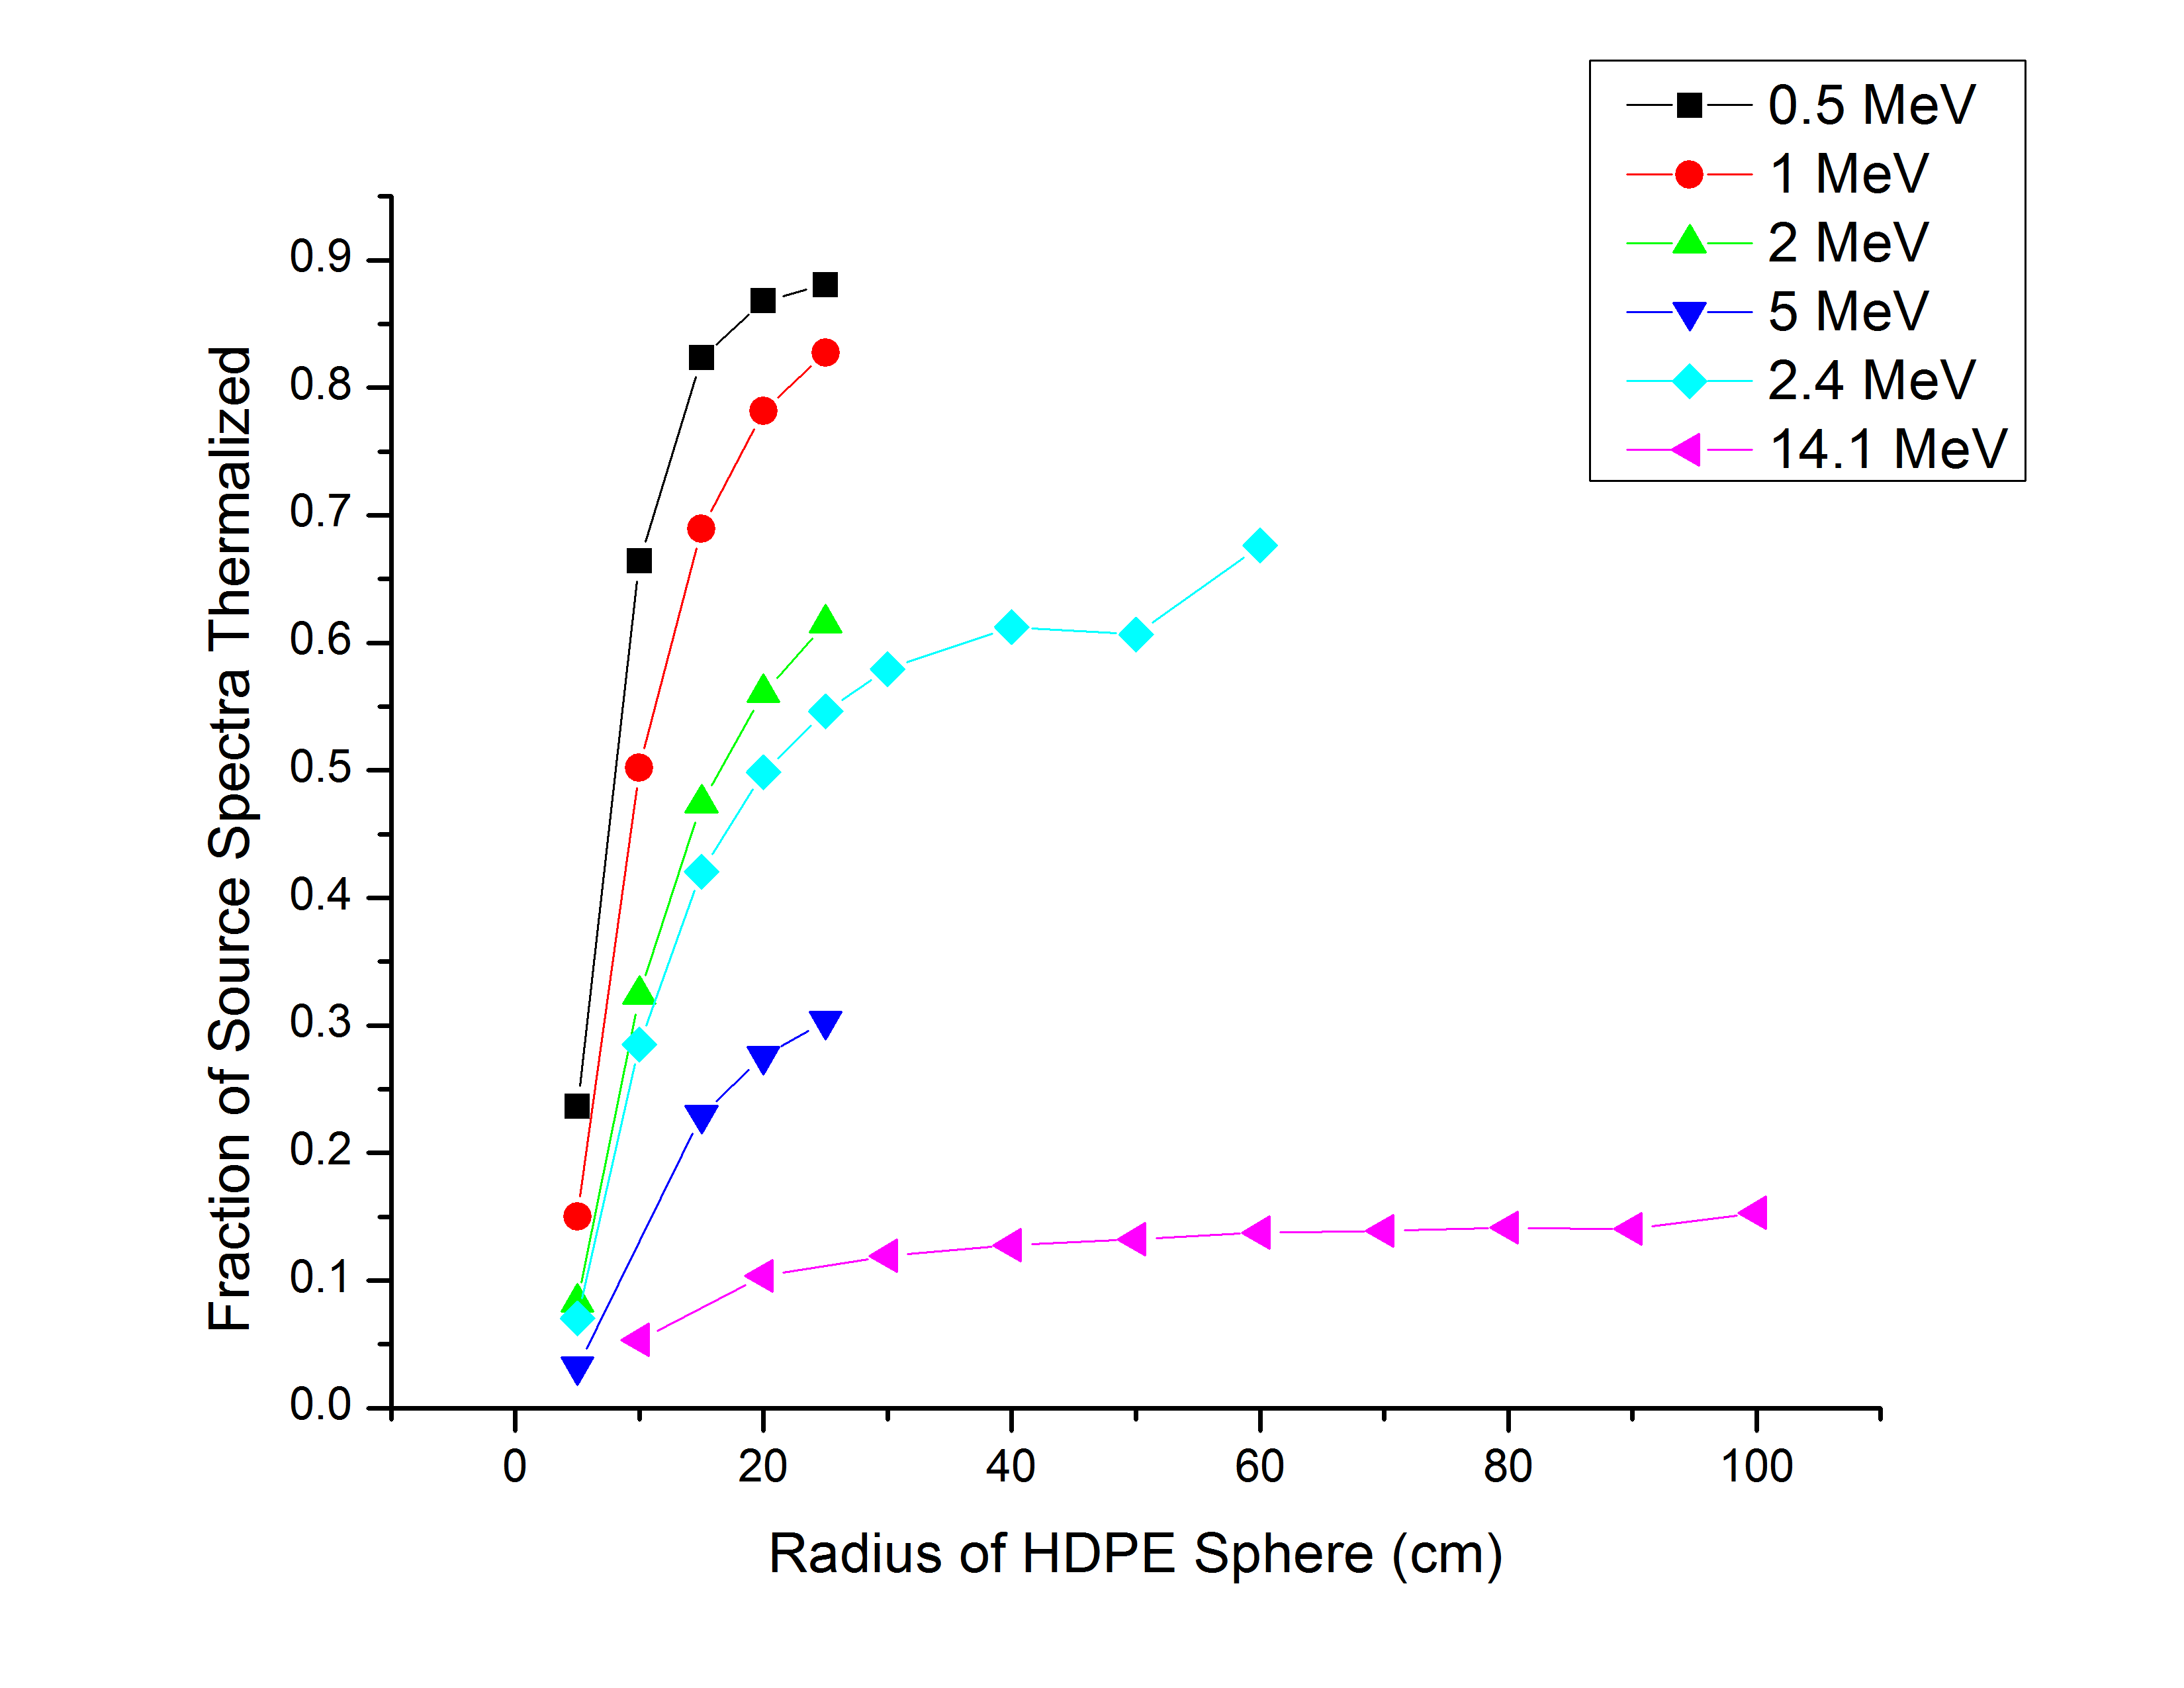
\includegraphics[width=0.5\textwidth]{FractionThermalized_EDep}
\caption{Fraction of Spectra Thermalized}
\label{fig:FractionThermalized}
\end{figure}
\subsection{Example Calculations}
The number of neutrons outside of the moderator can be calculated as follows:
For the 2.4 MeV source of strength $1.2\times10^{12} n/s$:
\begin{equation}
\eta = \frac{1.04266E-05}{1.54171E-05} = 0.67
\end{equation}
So 67\% of the neutrons leaving the 60 cm radius sphere of HDPE have an energy below $10^{-7}$ MeV. 
The total number of neutrons making it outside of the HDPE sphere is then:
\begin{equation}
1.2\times10^{12} n/s \cdot 1.54\times10^{-5} = 1.84\times10^{7} n/s
\end{equation}
Given that the sphere is 60 cm, the flux can be calculated at the surface of the sphere for both the thermal and total flux:
\begin{align}
    \Phi_{E\le10^{-7} MeV} &= \frac{1.2\times10^{12} n/s \cdot 1.042\times10^{-5}}{4\pi (60 cm)^2} \\
                           &= 276 \pm 52 n/cm^2 s 
\end{align}
\begin{align}
    \Phi_{Total} &= \frac{1.2\times10^{12} n/s \cdot 1.54\times10^{-5}}{4\pi (60 cm)^2} \\
                  &= 408 n/cm^2 s
\end{align}
This value can be compared to the MCNP calculated thermal flux at the surface of HDPE.
\begin{align}
    \Phi_{E\le10^{-7} MeV} &= 1.2\times10^{12} n/s \cdot  4.080 \times10^{-10} particles/cm^2\\
                           &= 489 \pm 107 n/cm^2s 
\end{align}
It follows that the F2 flux tally is slightly higher than the F1 current tally because the F1 tally is weighted by the do product of the particle direction and the surface normal, while the F2 tally does not.

The 14.1 D-T source had 5.63936E-03 neutrons per source neutron below 1E-7 MeV, with a total of 4.10137E-02 neutrons exiting the HDPE.
Using the definition of the thermal fraction from above, $\eta$ is
\begin{equation}
\eta = \frac{5.63936E-03}{4.10137E-02} = 0.137499
\end{equation}.
If the source strength is $3.5\times10^{14}$ n/s, then there would be $3.5\times10^{14} \cdot 5.63936\times10^{-3} = 1.97\times10^{12}$ n/s leaving the HDPE moderator (all $4\pi$ solid angle), or a flux of $\frac{1.97\times10^{12}}{4\pi (60 cm)^2} = 4.36\times10^{7} n/cm^2 s$ with an energy less than $10^{-7}$ MeV.

\section{Results}
The flux on the surface of the HDPE moderator sphere is shown in Figure ~\ref{fig:ThermalFluxSources} for both the D-T and D-D sources. The D-D source has a thermal flux within the design constraint of $106{7} n/cm^2s$ around a thickness of 25 cm, while the D-T source because of it's higher energy requires significantly more (95 cm) moderator to meet the design constraint.
\begin{figure}[ht]
    \centering
    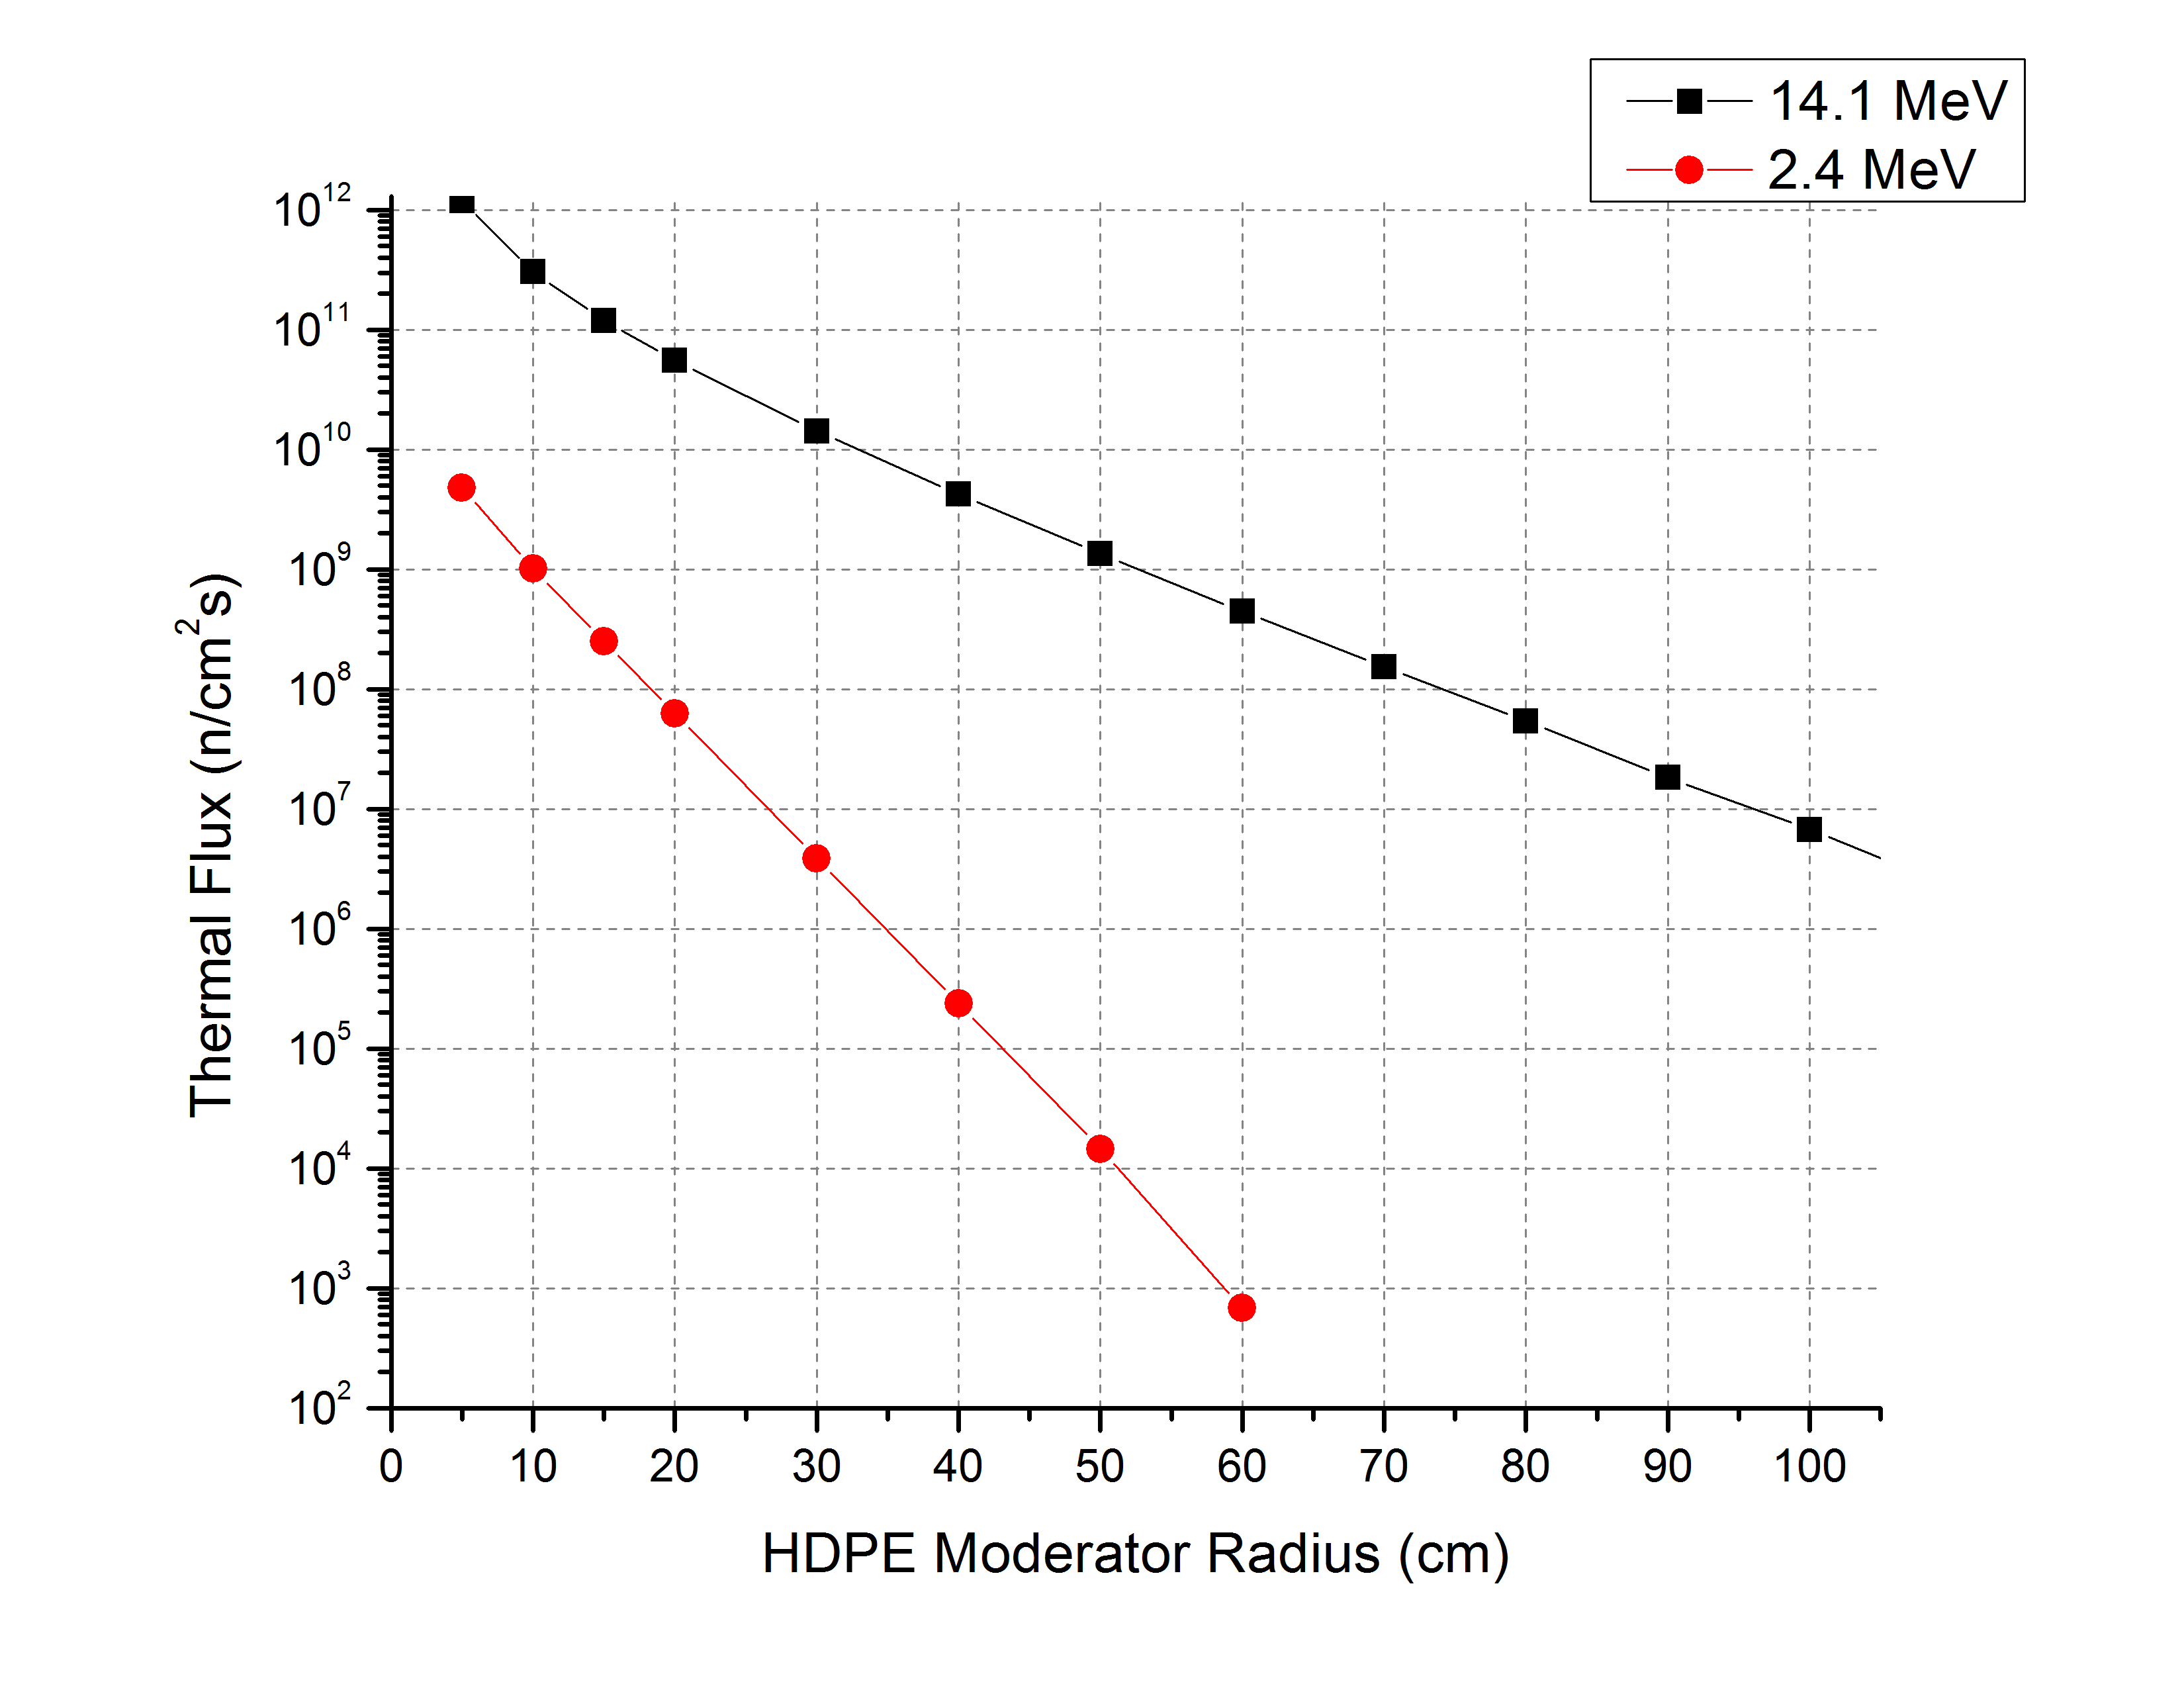
\includegraphics[width=0.5\textwidth]{ThermalFluxSources}
    \caption{Thermal flux as a function of HDPE Moderator Radius for the D-D and D-T sources}
    \label{fig:ThermalFluxSources}
\end{figure}
The fraction of thermal neutrons was calculated with both the F1 current tally and the F2 flux tallies, with good agreement, as shown in Figure ~\ref{fig:DDDTThermalFraction}. 
For the D-D source the thermal fraction is around 50\% with 25 cm of moderator, and for the D-T source the thermal fraction is only at 15\% with 95 cm of moderator.
\begin{figure*}[ht]
	\centering
	\begin{subfigure}[b]{0.43\textwidth}
		\centering
		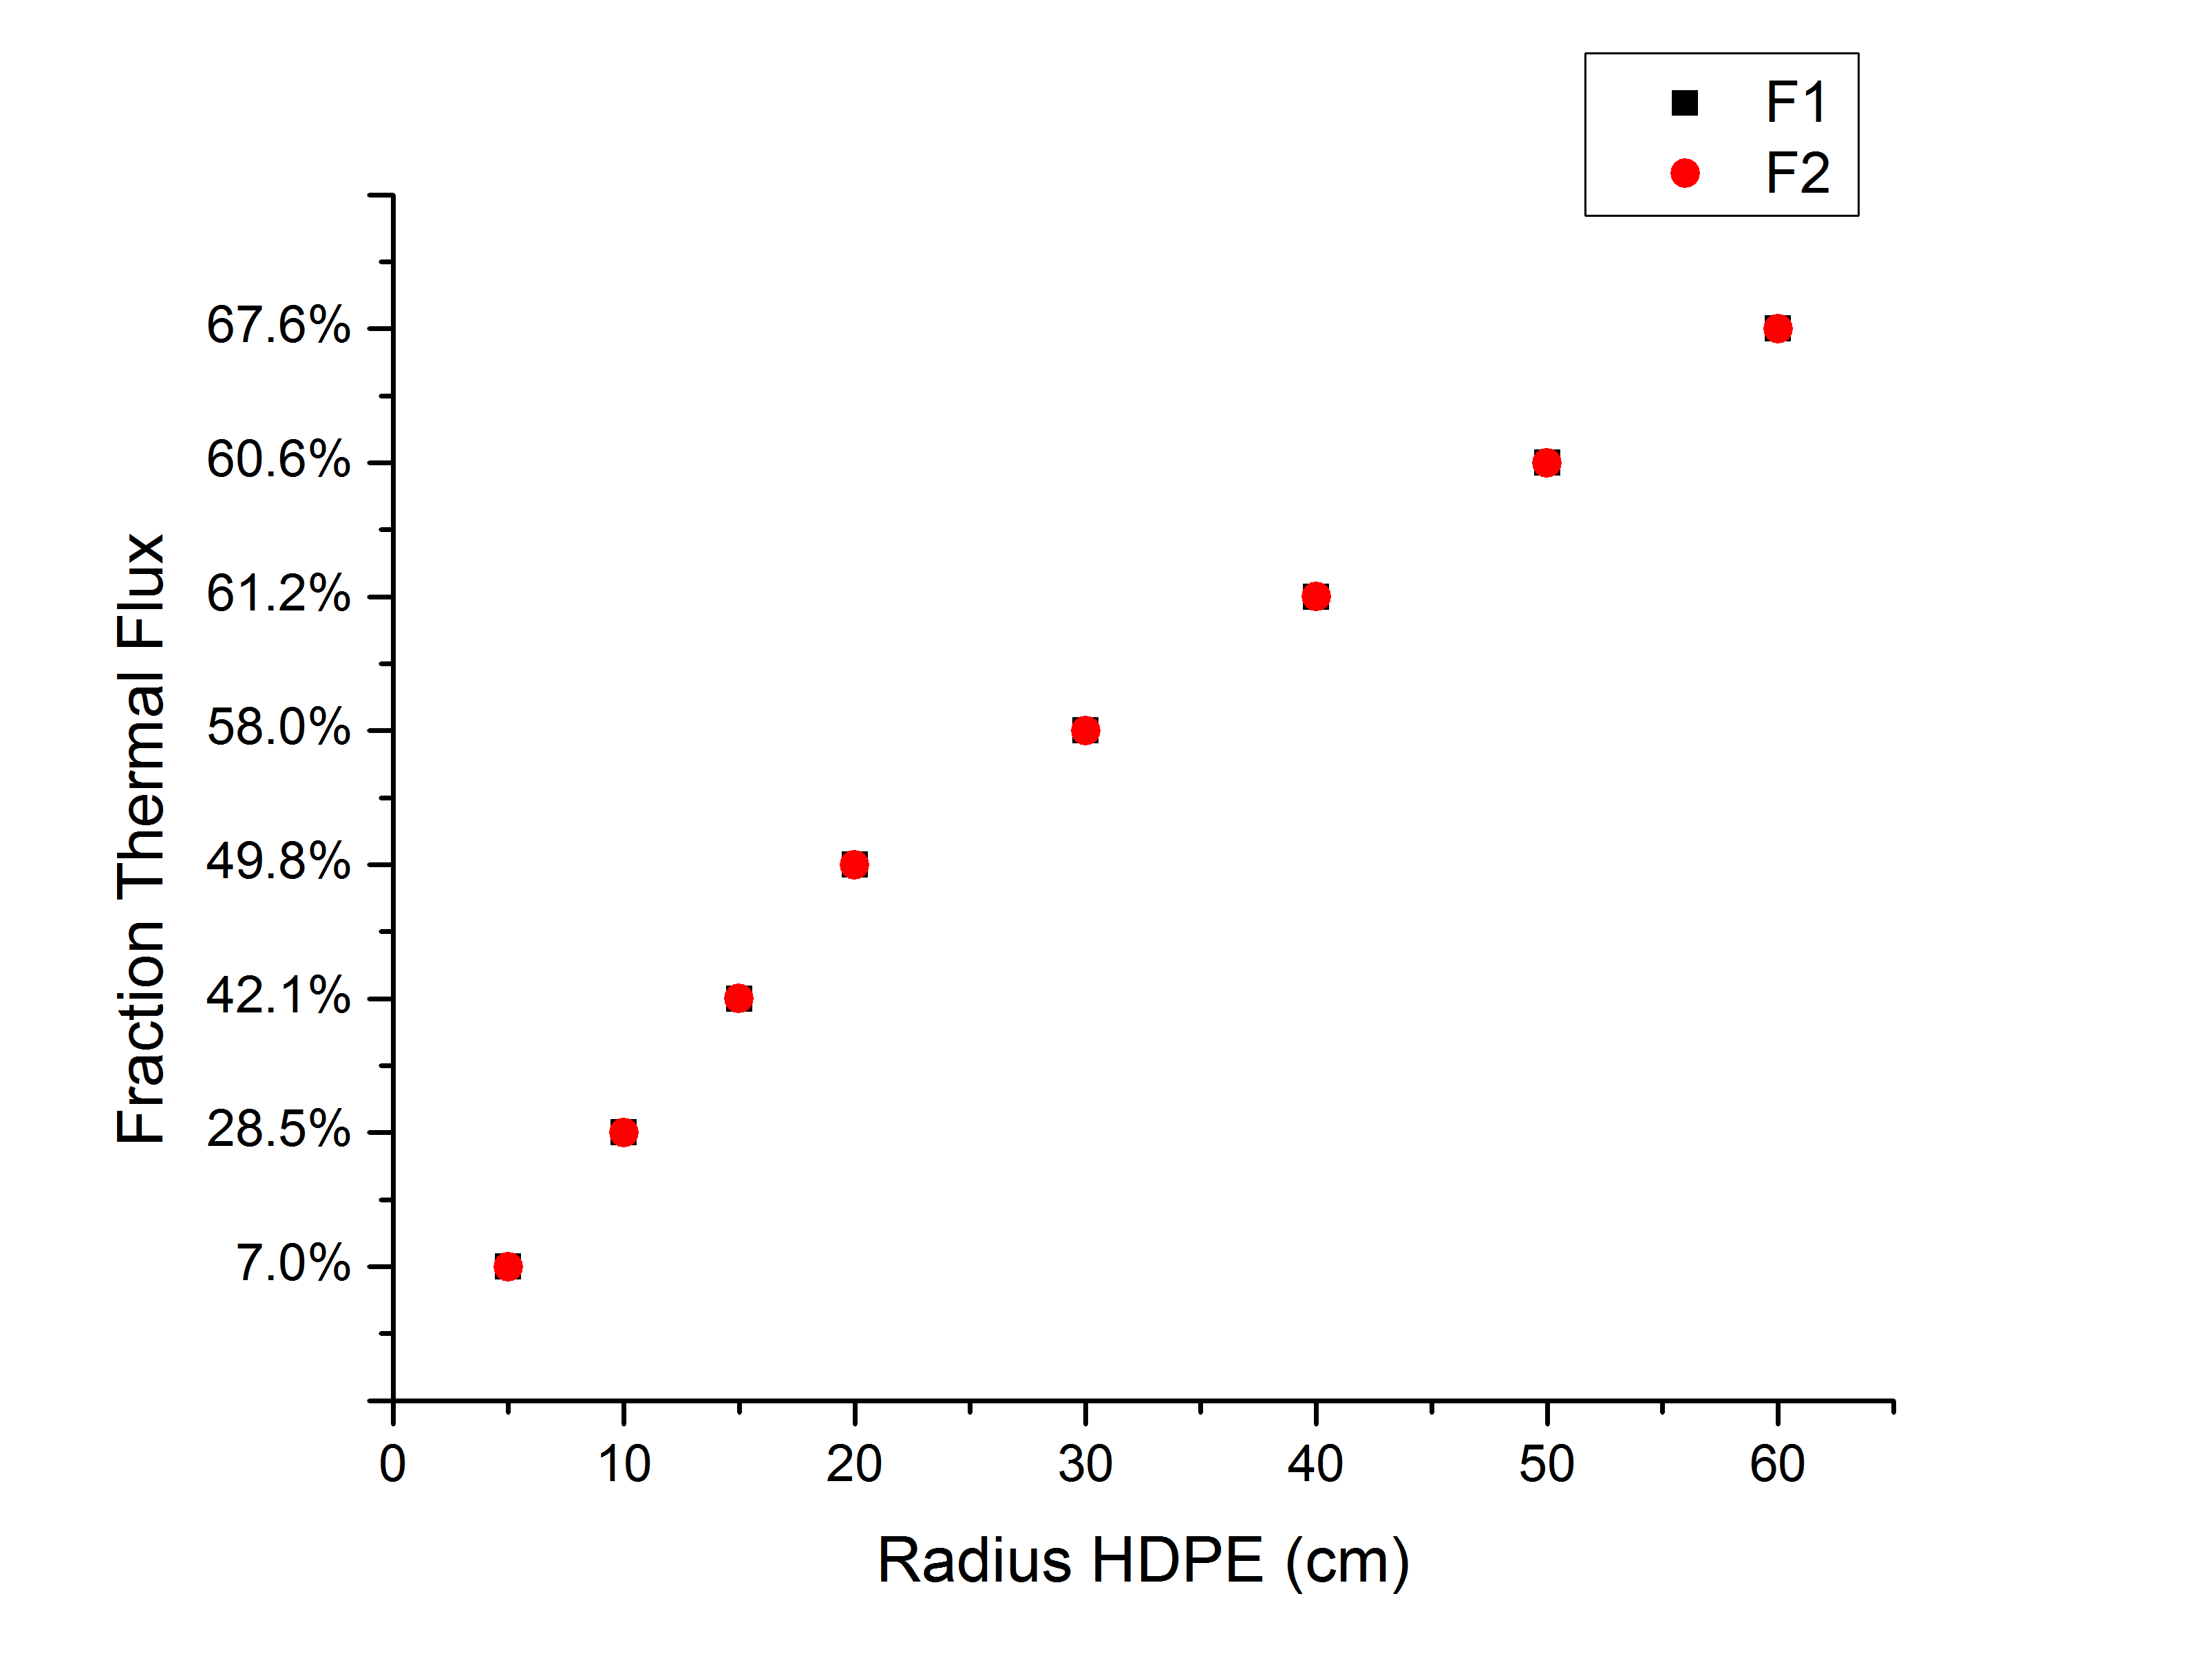
\includegraphics[width=\textwidth]{DDThermalFraction}
        \caption{D-D Thermal Fraction (2.4 MeV)}
	\end{subfigure}%
	~
	\begin{subfigure}[b]{0.43\textwidth}
		\centering
		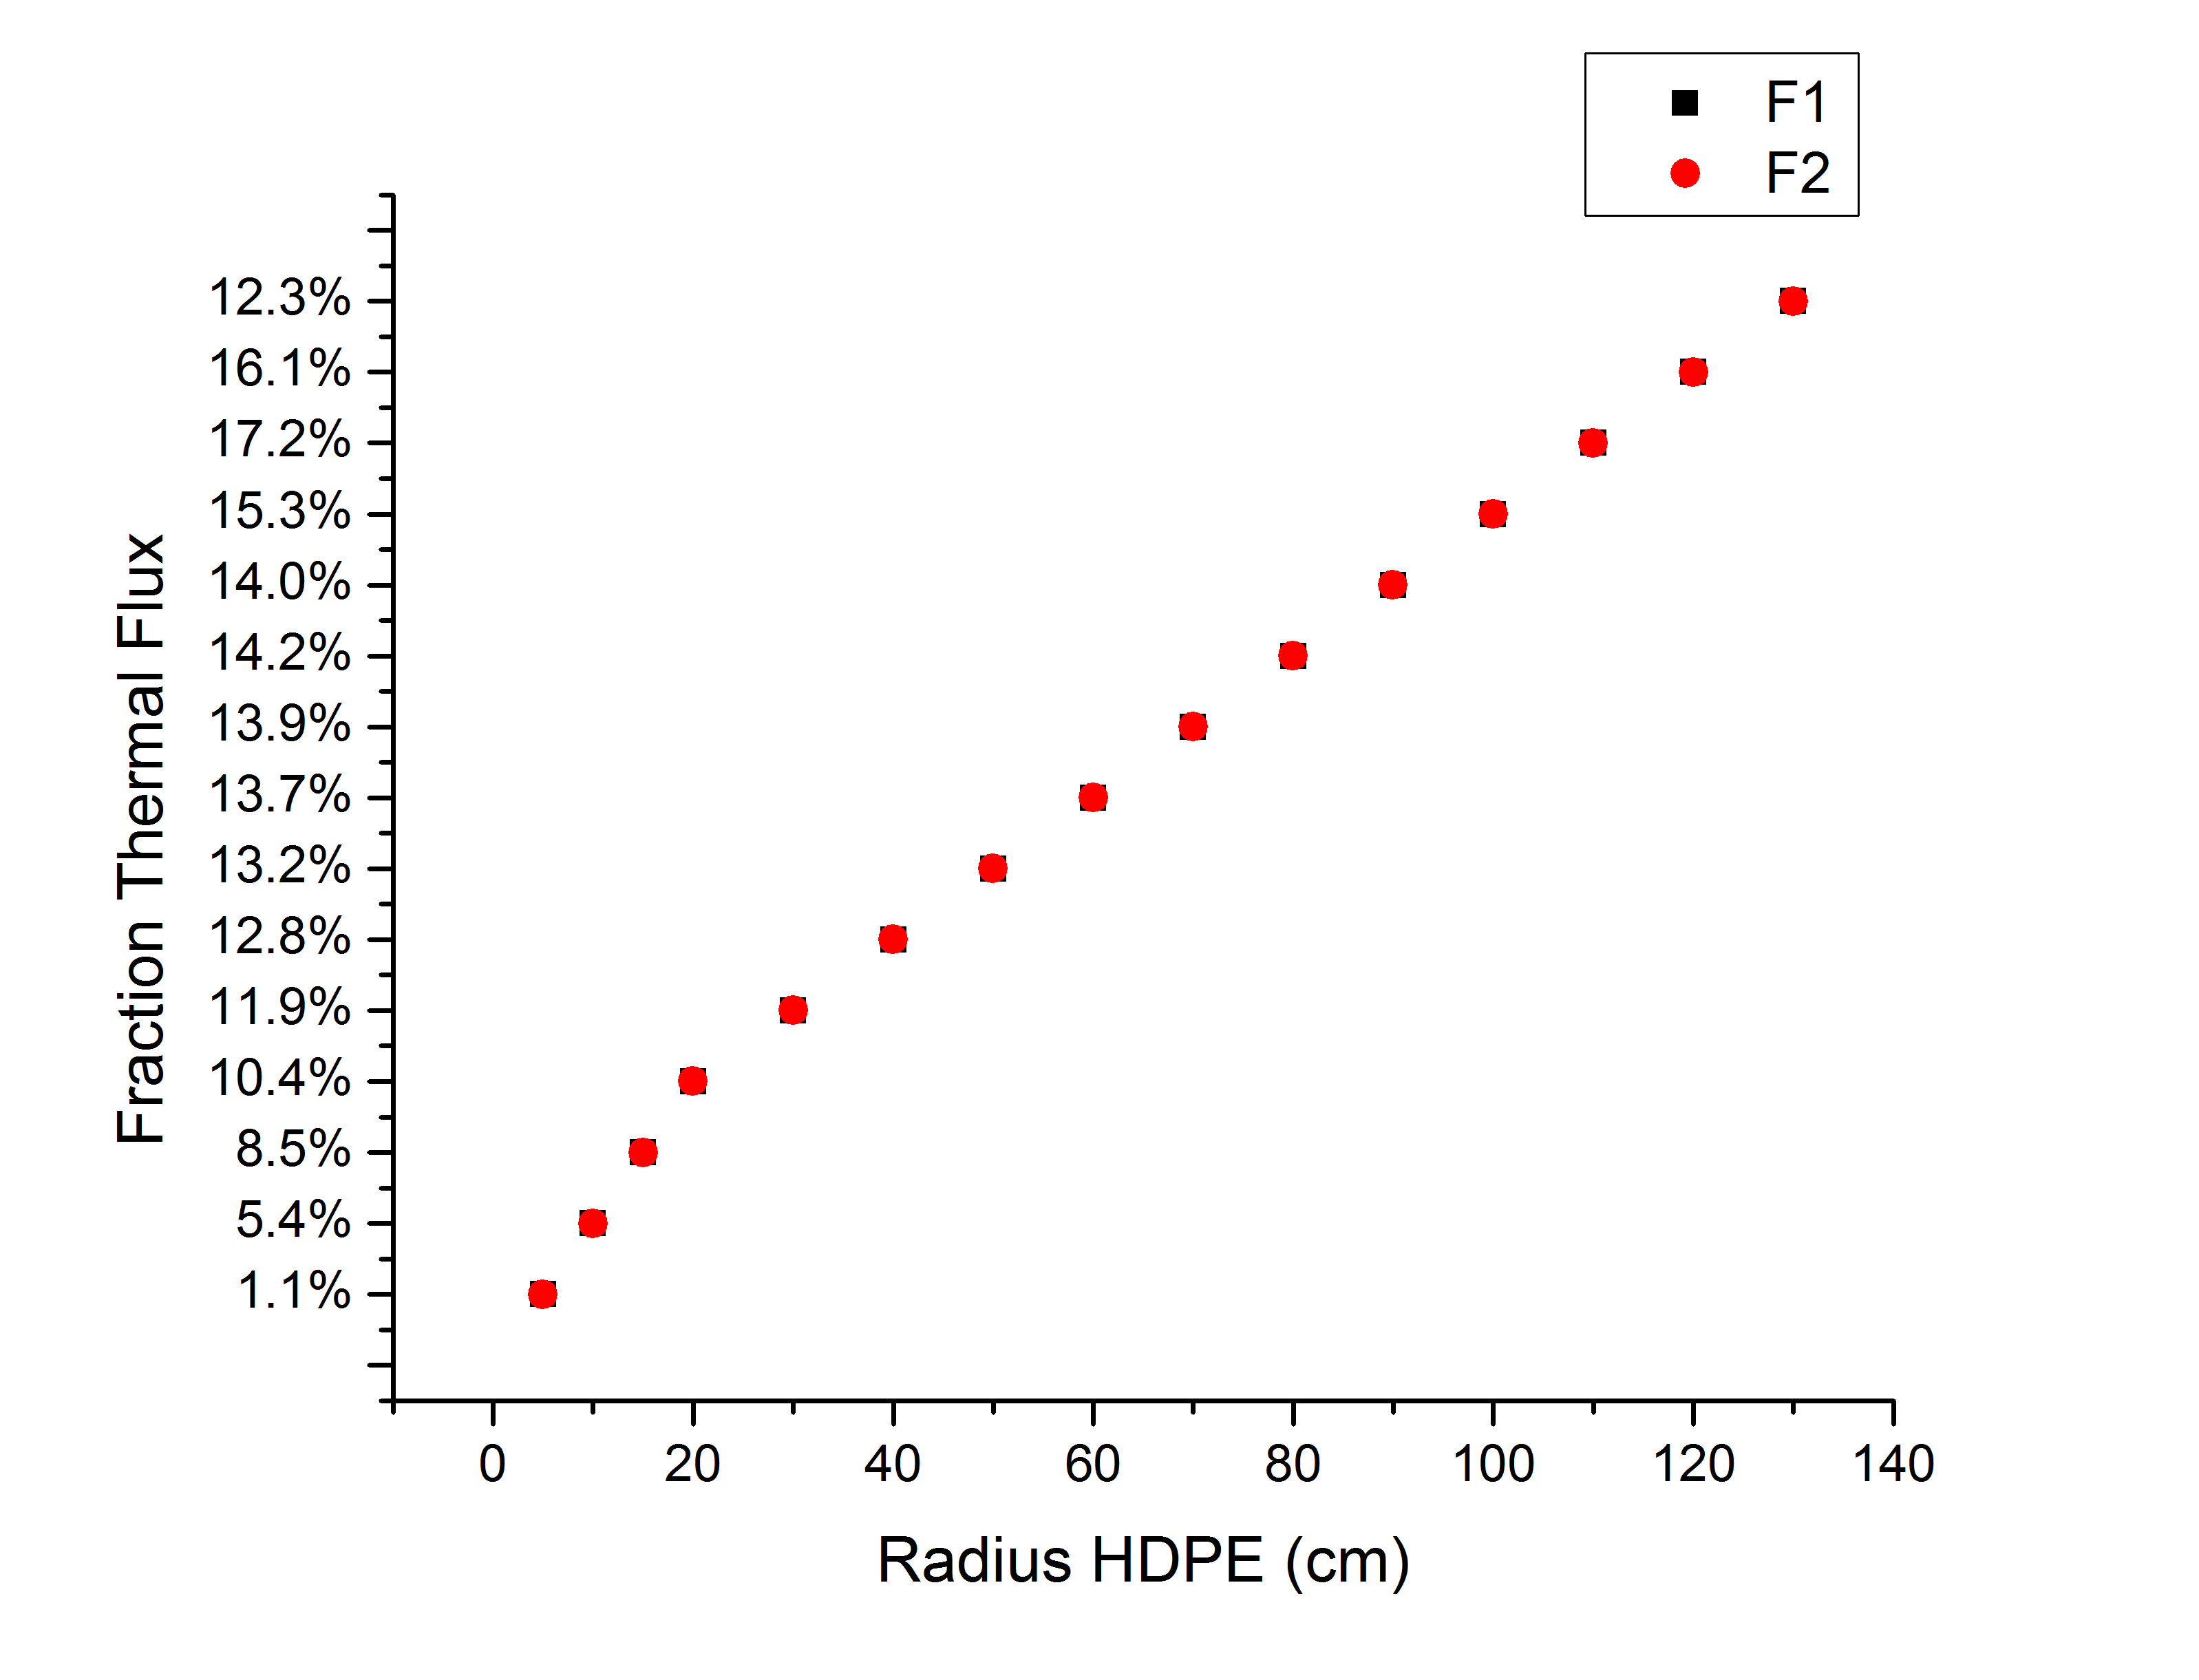
\includegraphics[width=\textwidth]{DTThermalFraction}
        \caption{D-T Thermal Fraction (14.1 MeV)}
	\end{subfigure}	
	\caption{Thermal fraction calculated by F1 and F2 tallies}
	\label{fig:DDDTThermalFraction}
\end{figure*}
% Bibliography
\bibliography{./Zotero}

\end{document}


%\includepdf[pages=-]{DTDDSheilding.pdf}

\end{document}

